\documentclass[10pt,a4paper]{article}

\usepackage[T1]{fontenc}
\usepackage[utf8]{inputenc}
\usepackage{ae}
\usepackage{aecompl}
\usepackage{zefonts}
\usepackage{multicol}
\usepackage{array, multirow, tabularx}
\usepackage{makecell}
\usepackage{graphicx}
% \usepackage{picins}
\usepackage{amsfonts,amsmath,amssymb}
\usepackage{eurosym}
\usepackage{ulem} %permet de barrer sdu texte avec \sout{} , hachurer avec \xout , souligner avec vaguelette \uwave
\usepackage{textcomp}
\usepackage{graphicx}
\usepackage{yhmath} %arc de cercle avec $\wideparen{AB}$
\usepackage[np]{numprint} %espacement grands nombres
\usepackage{fdsymbol} % symbole calculatrice casio
\usepackage{enumerate}
\usepackage{fancybox} % shadowbox etc...
\usepackage{pifont}
\usepackage{tabularx} 
\usepackage{boxedminipage}
\usepackage[thmmarks,framed]{ntheorem}   %fonction  \newtheorem améliorée incompatible avec amsthm
\usepackage{framed}
\usepackage{titlesec}
\usepackage{colortbl} %charge xcolor , à mettre avant tikz sinon conflit...
\usepackage{pgfkeys} % repères avec tikz
\usepackage{tikz}
\usepackage{tkz-tab} %tableaux de variation
\usepackage{esvect} %vecteurs
\usepackage{pgf} %exporter figures geogebra
\usepackage{mathrsfs} %exporter figures geogebra
\usepackage{slashbox} %sépare une cellule en 2 dans un tableau \backslashbox{Texte dessous}{Texte dessus}
\usepackage{diagbox} %\diagbox{}{}
\usetikzlibrary{arrows} %exporter figures geogebra
\usepackage[french,frenchkw,algoruled]{algorithm2e} %algo 
%\usepackage{algorithm} %algo style algobox
% \usepackage{algpseudocode}% algo style algobox
% \input algtolatex %algo style algobox - nécessite le fichier algolatex.
\usepackage{calrsfs} % plus belles majuscules avec \mathcal
% \usepackage{sesamanuel} % pour les commandes spéciales du manuel 2de
% \usepackage{sesamanuelTIKZ} % pour les commandes spéciales de la figure
%\usepackage{stmaryrd} %double crochet avec \llbracket et rrbracket$
\usepackage{qrcode} %qrcode cliquable \qrcode[height=taille]{adresse}
\usepackage{hyperref} %lien hypertexte \href{adresse}{texte}
%\usepackage[xcas]{pro-graphes} %graphe and co
%\usepackage{dijkstra}
\usepackage{tcolorbox} %cadres plus jolis
\usepackage{karnaugh-map} %permet de tracer des tableaux de Karnaugh
%\usepackage{graphicx}
\usepackage[export]{adjustbox} % Alignement vertical images avec b,t,c \includegraphics[scale=1,valign=t]{Image.png}
\usepackage{fancyvrb} % verbatim amélioré \begin{Verbatim}[frame=single,label=,numbers=left] etc [frame=single/leftline/topline/bottomline/lines] framerule=1mm framesep=5mm rulecolor=\color{red} fillcolor=\color{yellow}
\usepackage[load-configurations = abbreviations]{siunitx}
%\sisetup{locale = FR,detect-all,inter-unit-product= \cdot} %norme SI pour les nombres et unités 
%\SI{25000}{mm} \SI{6.022e23}{\per\mol}  \SI{300}{\watt\per\square\meter} \SI{300}{W / m^2} \SI[per-mode=symbol]{210}{\km\per\hour}
% unité seule \si{\newton\meter} nombre seul \num{24415.15625}

\usepackage{witharrows} %permet de mattre des flèches entre lignes d'équations \begin{WithArrows}@ \Arrow{@}\\@\end{WithArrows}

\usepackage{xlop} % pose les oprétaions "à la main" \opadd{@}{@}; opsub ; opmul ; opdiv (eucl) ; opidiv
%\usepackage{minted}{Python} % permet d'écrire en Python avec \begin{minted}{Python}@\end{minted}
\usepackage{stmaryrd} % crochets intervalles entiers \llbracket ; \rrbracket ; parall \sslash ; contradiction \lightning

\usepackage{mathtools}

%%%%%%%Compteurs%%%%%%%%%%%%%%%%%%%%%%%%%%%%%%%%%%%%%%%%%%%%%%%%%%%%%%%%%%%%%%%%%%%%%
% \newcounter{defcompt}   %Défintion d'un compteur
% \newcounter{exocompt}
% \newcounter{theocompt}
% \newcounter{propcompt}
% \newcounter{regcompt}
\newcounter{numexos}

\setcounter{numexos}{0} %initialisation du compteur





% Nouvelles commandes
\definecolor{cqcqcq}{rgb}{0.7529411764705882,0.7529411764705882,0.7529411764705882} %gris geogebra

\newcommand{\paral}{~\mathbin{\!/\mkern-5mu/\!}~} % symbole parallèle

\newcommand{\R}{\mathbb{R}}
\newcommand{\N}{\mathbb{N}}
\newcommand{\D}{\mathbb{D}}
\newcommand{\Z}{\mathbb{Z}}
\newcommand{\Q}{\mathbb{Q}}
\newcommand{\C}{\mathbb{C}}
\newcommand{\U}{\mathbb{U}}

\newcommand{\rel}{\mathcal{R}} % relation binaire

\newcommand{\e}{\text{e}} % exponentielle en lettre droite dans $$ 

\newcolumntype{R}[1]{>{\raggedleft\arraybackslash }b{#1}}
\newcolumntype{L}[1]{>{\raggedright\arraybackslash }b{#1}}
\newcolumntype{C}[1]{>{\centering\arraybackslash }b{#1}}

\newcolumntype{G}[1]{>{\raggedright\arraybackslash }X{#1}}
\newcolumntype{D}[1]{>{\raggedleft\arraybackslash }X{#1}}
\newcolumntype{M}[1]{>{\centering\arraybackslash }X{#1}}


\newcommand{\exe}{\textbf{Exemple : }}
\newcommand{\exes}{\textbf{Exemples : }}
\newcommand{\rema}{\textbf{Remarque : }}
\newcommand{\rems}{\textbf{Remarques : }}
\newcommand{\rap}{\textbf{Rappel : }}
\newcommand{\raps}{\textbf{Rappels : }}
\newcommand{\dem}{\textbf{Démonstration : }}
\newcommand{\dems}{\textbf{Démonstrations : }}
\newcommand{\csq}{\textbf{Conséquence : }}







\newcommand{\Ex}[1]{{\sc{Exercice #1:}}}
\newcommand{\defi}[1]{\begin{leftbar}
\textbf{Définition :} {#1}
 \end{leftbar}}
\newcommand{\defis}[1]{\begin{leftbar}
\textbf{Définitions :} {#1}
 \end{leftbar}}
 
\newcommand{\prop}[1]{\begin{framed}
\textbf{Propriété :} {#1}
 \end{framed}} 
 
\newcommand{\props}[1]{\begin{framed}
\textbf{Propriétés :} {#1}
 \end{framed}} 
 
\newcommand{\theo}[1]{\begin{framed}
\textbf{Théorème :} {#1}
 \end{framed}} 
\newcommand{\theos}[1]{\begin{framed}
\textbf{Théorèmes :} {#1}
 \end{framed}}  
 
\newcommand{\reg}[1]{\begin{framed}
\textbf{Règle :} {#1}
 \end{framed}} 
\newcommand{\regs}[1]{\begin{framed}
\textbf{Règles :} {#1}
 \end{framed}}  
 
\newcommand{\propdef}[1]{\begin{framed}
\textbf{Propriété - Définition :} {#1}
 \end{framed}} 
\newcommand{\propsdef}[1]{\begin{framed}
\textbf{Propriétés - Définition :} {#1}
 \end{framed}}  
 
 
 \newcommand{\csqs}[1]{\begin{framed}
 \textbf{Conséquences :} {#1}
 \end{framed}} 
 
\newcommand{\cor}[1]{\begin{framed}
\textbf{Corollaire :} {#1}
 \end{framed}}     
     
     
%\newcommand{\cadre}[2]{
%\begin{tcolorbox}[colback=red!5!white,
%                  colframe=red!75!black,
%                  title={#1}]
%{#2}
%\end{tcolorbox}  }

\newcommand{\cadre}[3]{
\begin{tcolorbox}[colback=#1!5!white,
                  colframe=#1!75!black,
                  title={#2}]
{#3}
\end{tcolorbox}  }




\newcommand*{\Coord}[3]{% 
\ensuremath{\vv{#1}\, 
    \begin{pmatrix} 
      #2\\ 
      #3 
    \end{pmatrix}}} % coordonnées de vecteurs.
    
\newcommand{\fonction}[5]{\begin{tabular}[t]{cccc}
$#1 :$ & $#2$ & $\longrightarrow$ & $#3$ \\
 & $#4$ & $\longmapsto$ & $#5$
\end{tabular}}
    
\newcommand{\att}{{\fontencoding{U}\fontfamily{futs}\selectfont\char 66\relax \quad}}    % symbole attention

\newcommand{\exo}{%Création d'une macro ayant un paramètre
\addtocounter{numexos}{1}%chaque fois que cette macro est appelée, elle ajoute 1 au compteur numexos
{\sc{Exercice\,\thenumexos\,:}}\,%la valeur du compteur appelée par \thenumeexos
}

\newcommand{\bint}{\displaystyle \int\limits} %signe intégral plus grand

\newcommand{\bsum}{\displaystyle \sum} %signe somme plus grand

\newcommand{\bprod}{\displaystyle \prod\limits} %signe produit plus grand

\newcommand*{\norme}[1]{\left\lVert\vv{#1}\right\rVert}  %norme de vecteur

\newcommand{\ps}[2]{\ensuremath{\vv{#1}.\vv{#2}}} %produit scalaire

\newcommand{\x}{\times} %produit

\newcommand{\modulo}{\text{ modulo }} 

\renewcommand{\Im}[1]{\text{Im} (#1)}

\renewcommand{\Re}[1]{\text{Re} (#1)}

\newcommand{\modu}[3]{{#1} \equiv {#2} ~ [{#3}]}


\newcommand*{\sep}[1]{
\dotfill
\vspace*{-0.3cm}
\begin{center}
\textbf{#1}
\end{center}
\vspace*{-0.5cm}
\dotfill}


%Flèches avec commentaire : exemple $\xRightarrow[test1]{test1}$
%\makeatletter
%\newcommand{\xRightarrow}[2][]{\ext@arrow 0359\Rightarrowfill@{#1}{#2}}
%\makeatother
%
%\makeatletter
%\newcommand{\xLeftarrow}[2][]{\ext@arrow 0359\Leftarrowfill@{#1}{#2}}
%\makeatother
%
%\makeatletter
%\newcommand{\xLeftrightarrow}[2][]{\ext@arrow 0359\Leftrightarrowfill@{#1}{#2}}
%\makeatother


% Renouvellement commandes

\renewcommand{\leq}{\leqslant}
\renewcommand{\geq}{\geqslant}
\renewcommand{\thesection}{\Roman{section} )  \hspace{-4mm}}
\renewcommand{\thesubsection}{\quad \arabic{subsection}\hspace{-0.9mm} ) \hspace{-5mm}}
\renewcommand{\thesubsubsection}{\qquad \alph{subsubsection}\hspace{0.5mm} ) \hspace{-5mm}}


% Présentation générale

\newcommand{\titre}[1]{\begin{center} \Large \sc \fbox{{#1}}\end{center}}

\newcommand{\entete}[1]{\begin{center} \large \underline{#1} \end{center}}

\titleformat*{\section}{\large\bfseries}
\titleformat*{\subsection}{\large\bfseries}
\titleformat*{\subsubsection}{\large\bfseries}
\titleformat*{\paragraph}{\large\bfseries}
\titleformat*{\subparagraph}{\large\bfseries}

%\newcommand{\DS}[3]{\begin{tabular}{|L{6cm}|C{5cm}|C{6cm}|}
%\hline 
%Nom : & Devoir Surveillé #1 & Classe \quad :\quad #2 \\ 
%Prénom : &  & #3 \\ 
%\hline 
%\end{tabular} }

\newcommand{\DS}[3]{\begin{tabularx}{1 \linewidth}{|G|M|M|}
\hline 
Nom : & Devoir Surveillé #1 & Classe \quad :\quad #2 \\ 
Prénom : &  & #3 \\ 
\hline 
\end{tabularx} }

\newcommand{\DSBTS}[4]{\begin{tabularx}{1 \linewidth}{|G|M|M|}
\hline 
Nom : & Devoir Surveillé #2 & Classe \quad :\quad #3 \\ 
Prénom : & #1 & #4 \\ 
\hline 
\end{tabularx} }

\newcommand{\DM}[3]{\begin{tabular}{|L{6.1cm}|C{5.6cm}|C{6.1cm}|}
\hline 
Nom : & Devoir à la maison~ #1 & Classe \quad :\quad #2 \\ 
Prénom : &  & Pour le #3 \\ 
\hline 
\end{tabular} }

\newcommand{\ct}[3]{\begin{tabular}{|L{6.1cm}|C{5.6cm}|C{6.1cm}|}
\hline 
Nom : & Contrôle~ #1 & Classe \quad :\quad #2 \\ 
Prénom : &  & #3 \\ 
\hline 
\end{tabular} }

% Repères automatisés avec Tikz 
% Définition des nouvelles options xmin, xmax, ymin, ymax
% Valeurs par défaut : -3, 3, -3, 3
\tikzset{
xmin/.store in=\xmin, xmin/.default=-3, xmin=-3,
xmax/.store in=\xmax, xmax/.default=3, xmax=3,
ymin/.store in=\ymin, ymin/.default=-3, ymin=-3,
ymax/.store in=\ymax, ymax/.default=3, ymax=3,
}
% Commande qui trace la grille entre (xmin,ymin) et (xmax,ymax)
\newcommand {\grille}
{\draw[help lines] (\xmin,\ymin) grid (\xmax,\ymax);}
% Commande \axes
\newcommand {\axes} {
\draw[->] (\xmin,0) -- (\xmax,0);
\draw[->] (0,\ymin) -- (0,\ymax);
}
% Commande qui limite l’affichage à (xmin,ymin) et (xmax,ymax)
\newcommand {\fenetre}
{\clip (\xmin,\ymin) rectangle (\xmax,\ymax);}

% Exemple 
%\begin{center}
%\begin{tikzpicture} [xmin=@,xmax=@,ymin=@,ymax=@]
%\grille \axes \fenetre
%\draw plot[smooth] (\x,@);
%\end{tikzpicture}
%\end{center}

%%%%%%%\newtheorem{}{×}%%%%%%%%%%%%%%%%%%%%%%%%%%%%%%%%%%%%%%%%%%%%%%%%%%%%%%%%%%%%%
%\theoremseparator{\hspace{0.8mm} :}
%{\theoremseparator{~:}
%\newtheorem*{rem}{Remarque}
%\newtheorem*{rems}{Remarques}
%\newframedtheorem{theo}[theocompt]{Théorème}
%\newtheorem{prop}[propcompt]{Propriété}
%\newtheorem{regle}[regcompt]{Règle}
%\newtheorem{defi}[defcompt]{Définition}
%\newtheorem*{voc}{Vocabulaire}}


%algo
%VARIABLES : 
%\Variables
%Début et fin de bloc :
%\DebutAlgo 
%\FinAlgo 
%\DebutPour
%\FinPour
%\DebutTantQue
%\FinTantQue
%\DebutSi
%\FinSi
%\DebutSinon
%\FinSinon
%SI...ALORS :
%\Si{(...)}
%SINON :
%\Sinon
%POUR ... ALLANT_DE ... A ...
%\Pour{...}{...}{...}
%TANT_QUE(...)
%\Tantque{(...)}
%Pour toutes les autres instructions (y compris les déclarations de variable)
%\Ligne ...


% Mise en page
\usepackage[left=1cm, right=1cm, top=1cm , bottom=1cm]{geometry}
\pagestyle{empty} % pas de numéro de page
\renewcommand{\arraystretch}{1.5} %hauteur des lignes dans un tableau
\setlength{\parindent}{0pt} % pas de retrait de paragraphe

%\usepackage[left=1cm, right=1cm, top=-0.5cm , bottom=1cm,includeheadfoot]{geometry}
%\usepackage{fancyhdr}
%\pagestyle{fancy}

%\renewcommand{\headrulewidth}{1pt}
%\fancyhead[C]{\textbf{page \thepage}} 
%\fancyhead[L]{\leftmark}
%\fancyhead[R]{machin}

%\renewcommand{\footrulewidth}{1pt}
%\fancyfoot[C]{\textbf{page \thepage}} 
%\fancyfoot[L]{truc}
%\fancyfoot[R]{\leftmark}

% \tikz[baseline=(letter.base)]\node[draw,circle,inner sep=1pt] (letter) {B} %lettre entourée

%\usepackage{qrcode}
\begin{document}


\titre{Les nombres complexes : point de vue géométrique}

Dans tout le chapitre, on munit le plan d'un repère $(O,\vv{u},\vv{v})$ orthonormé direct .

\section{Représentation dans le plan complexe}

\subsection{Définitions}

\begin{minipage}{0.6 \linewidth}
\defis{À tout nombre complexe $z = a + ib$, avec $a$ et $b$ réels, on peut associer :

\begin{enumerate}[\quad $\bullet$]
\item L'unique point $M(a ; b)$. $M$ est appelé point image de $z$.
\item L'unique vecteur $\Coord{w}{a}{b}$. $\vv{w}$ est appelé vecteur image de $z$.
\end{enumerate}


Réciproquement :

\begin{enumerate}[\quad $\bullet$]
\item À tout point $M(a ; b)$ avec $a$ et $b$ deux réels, on peut associer l'unique nombre complexe $z = a + ib$.

Le nombre $z$ est appelé affixe du point $M$
\item À tout vecteur vecteur $\Coord{w}{a}{b}$ avec $a$ et $b$ deux réels, on peut associer l'unique nombre complexe $z = a + ib$.

Le nombre $z$ est appelé affixe du vecteur $\vv{w}$.
\end{enumerate}
}
\end{minipage}
\begin{minipage}{0.35\linewidth}
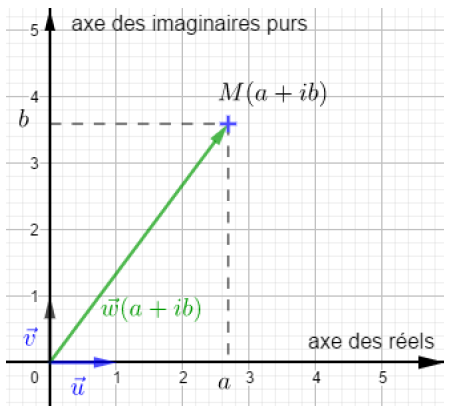
\includegraphics[width = 1 \linewidth]{cplx_rep_graph.png}
\end{minipage}

\medskip

\rems
\begin{enumerate}[$\bullet$]
\item Les nombres réels sont les affixes des points de l'axe des abscisses aussi appelé : axe des réels.
\item Les nombres imaginaires purs sont les affixes des points de l'axe des ordonnées aussi appelé : axe des imaginaires purs.
\item Lorsqu'un point ou un vecteur est repéré par son affixe, le plan est appelé le plan complexe.
\item L'affixe de $M$ est souvent noté $z_M$ et la donnée d'un point $M$ d'affixe $z_M$ est souvent notée $M(z_M)$.

L'affixe de $\vv{w}$ est souvent noté $z_{\vv{w}}$, et la donnée d'un vecteur $w$ d'affixe $z_{\vv{w}}$ est souvent notée 
$ \vv{w}(z_{\vv{w}})$ .

\end{enumerate}

\exes $A(1;2)$ avec $z_A=1+2i$. $z_{\vv{w}}=2-3i$ et $\Coord{w}{2}{-3}$.


\subsection{Propriétés}

Des propriétés connues de géométrie sur les vecteurs et points donnent les propriétés suivantes.

\props { Soient $A(z_A)$ et $B(z_B)$ deux points du plan complexe. Soient $ \vv{w_1}(z_{\vv{w_1}})$ et $ \vv{w_2}(z_{\vv{w_2}})$  deux vecteurs du plan complexe. Soit $\lambda \in \R$.

\vspace*{-0.4 cm}

\begin{multicols}{2}
\begin{enumerate}[$(i)$]
\item $A=B \iff z_A=z_B$ . 
\item $\vv{w_1}=\vv{w_2} \iff z_{\vv{w_1}}=z_{\vv{w_2}}$.
\item $\vv{AB}$ a pour affixe $z_B-z_A$.
\item Le milieu du segment $[AB]$ a pour affixe $\dfrac{z_A+z_B}{2}$.
\item Le vecteur $\vv{w_1}+\vv{w_2}$ a pour affixe $z_1+z_2$.
\item $\lambda \vv{w_1}$ a pour affixe $\lambda z_1$.
\end{enumerate}
\end{multicols}
}

\dem $(iii)$ On sait que $\Coord{AB}{x_B-x_A}{y_B-y_A}$ d'où pour les affixes :

$z_{\vv{AB}}=(x_B-x_A)+i(y_B-y_A)=(x_B-iy_B) - (x_A-iy_A)=z_B-z_A$. \medskip

\exe Soit $A(3 + 2i)$ et $B(5 - i)$. Alors le vecteur $\vv{AB}$ a pour affixe $z_{\vv{AB}} = 5 - i - (3 + 2i) = 2 - 3i$.

\begin{minipage}{0.6 \linewidth}
\subsection{Conjugué et opposé}

Les points $M$ d'affixe $z$ et $M'$ d'affixe $\overline{z}$ sont symétriques par rapport à l'axe des réels.

Les points $M$ d'affixe $z$ et $M''$ d'affixe $-z$ sont symétriques par rapport à l'origine du repère.
\end{minipage}
\begin{minipage}{0.35 \linewidth}
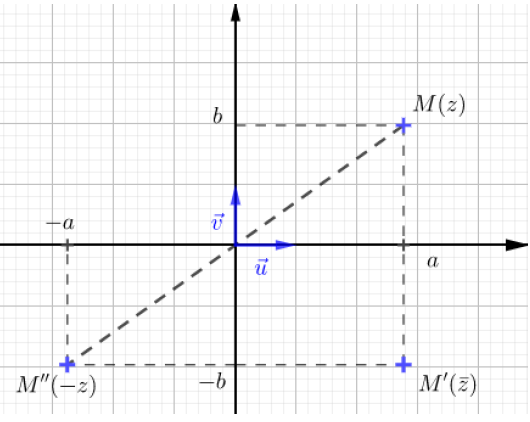
\includegraphics[width = 0.9 \linewidth]{cplx_sym.png}
\end{minipage}


\begin{minipage}{0.6 \linewidth}

\section{Module et argument d'un nombre complexe}


\subsection{Module}

\defi{Soit $M$ un point d'affixe $z$. Le module de $z$, noté $|z|$ est le réel positif défini par $|z| = OM$.

Si $z = a + ib$ avec $a$ et $b$ deux réels. Alors $|z| = \sqrt{a^2 + b^2}$.
}
\end{minipage}
\begin{minipage}{0.35 \linewidth}
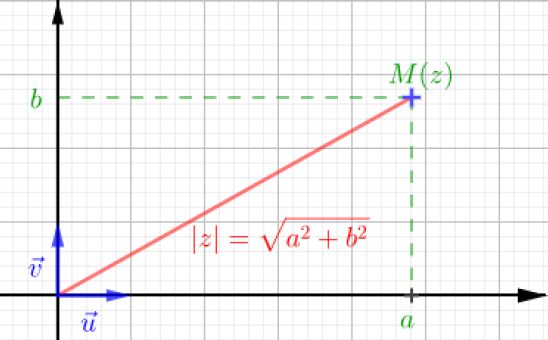
\includegraphics[width = 1 \linewidth]{cplx_mod}
\end{minipage}

\rema Si $z = z'$, alors $|z| = |z'|$. Mais la réciproque est fausse.

Contre-exemple avec $z=1+i$ et $z'=1-i$. $|z|=|z'|=\sqrt{2}$ et $z \neq z'$.


\props { Soit $z$ un nombre complexe. \vspace*{-0.3cm}
\begin{multicols}{3}
\begin{enumerate}[$(i)$]
\item $|z|^2=z \overline{z}$
\item $|\overline{z}|=|z|$
\item $|-z|=|z|$
\item $|z|=0 \iff z=0$
\end{enumerate}
\end{multicols}\vspace*{-0.3cm}
}

\dem

\begin{enumerate}[$(i)$]
\item $z \overline{z}=(a+ib)(a-ib)=a^2-(ib)^2=a^2-i^2b^2=a^2+b^2=|z|^2$
\item $|\overline{z}|=\sqrt{a^2+(-b)^2}=\sqrt{a^2+b^2}=|z|$
\item $|-z|=\sqrt{(-a)^2+(-b)^2}=\sqrt{a^2+b^2}=|z|$
\item $|z|=0 \Rightarrow a^2+b^2=0 \iff a=b=0$. Sens réciproque évident.
\end{enumerate}

\medskip

\rema Corollaire de (i) : \raisebox{-3.5mm}{\shadowbox{$|z|= \sqrt{z \overline{z}}$}}. (utile en pratique).

\prop{Soit $A(z_A)$ et $B(z_B)$. On a $AB = |z_B - z_A| = |z_A - z_B|$. 
}

\dem On a $AB=\norme{AB}=|z_{\vv{AB}}|=|z_B-z_A|$.

\props{Soient $z$ et $z'$ deux nombres complexes non nuls et entier naturel non nul.

\begin{multicols}{3}
\begin{enumerate}[$(i)$]
\item Produit : $|zz'|=|z||z'|$
\item Puissance : $|z^n|=|z|^n$  
\item Inverse : $\left| \dfrac{1}{z} \right|=\dfrac{1}{|z|}$
\item Quotient : $\left| \dfrac{z}{z'} \right|=\dfrac{|z|}{|z'|}$ 
\end{enumerate}
\end{multicols}

}



\dem

$\bullet$ Module d'un produit :$|zz'|^2=zz' \x \overline{zz'}= zz' \overline{z} \overline{z'}=z \overline{z} \x z'\overline{z'} = |z|^2 |z'|^2=(|z||z'|)^2$.

Or $|zz'| \in \R^+$ et $|z||z'| \in \R^+$ d'où $|zz'|=|z||z'|$

$\bullet$  Module d'une puissance : On procède par récurrence.

Initialisation : $|z^1|=|z|=|z|^1$. $P(1)$ est vraie.

Hérédité : Supposons qu'il existe un entier $k$ tel que la propriété $P(k)$ soit vraie : $|z^k|=|z|^k$

$|z^{k+1}|=|z^kz|=|z^k||z|=|z|^k|z|=|z|^{k+1}$

Conclusion : La propriété est vraie pour $n=1$ et héréditaire à partir de ce rang.

Donc elle est vraie pour tout entier naturel $n$, soit : $|z^n|=|z|^n$.

$\bullet$  Module de l'inverse :  $z \x \dfrac{1}{z}=1$ d'où $\left|z \x \dfrac{1}{z} \right|=|1|=1$ puis
$|z| \x \left| \dfrac{1}{z} \right| = 1 \iff \left| \dfrac{1}{z} \right| = \dfrac{1}{|z|}$.


$\bullet$  Module du quotient : $ \dfrac{z}{z'}= z \x \dfrac{1}{z'}$. Donc $\left| \dfrac{z}{z'}\right|=\left|z \x \dfrac{1}{z'} \right|=|z| \x \left| \dfrac{1}{z'} \right| = |z| \x \dfrac{1}{|z'|}= \dfrac{|z|}{|z'|}$.

\medskip

\prop{\textbf{Inégalité triangulaire}

Soient $z$ et $z'$ deux nombres complexes, on a $|z+z'| \leq |z|+|z'|$}

\dem Voir fiche complément

\subsection{Argument}

\begin{minipage}{0.6 \linewidth}
\defi{Soit un point $M$ d'affixe non nulle $z$.

On appelle argument de $z$, noté $\arg(z)$ une mesure, en radians, de l'angle $(\vv{u};OM)$.

}

\rems
\begin{enumerate}[$\bullet$]
\item Un nombre complexe non nul possède une infinité d'arguments de la forme $\arg(z) + 2k \pi, k \in \Z$.

On notera $\arg(z)$ modulo $2 \pi$ ou $\arg(z) [2\pi]$

\item 0 n'a pas d'argument car dans ce cas l'angle $(\vv{u};OM)$ n'est pas défini.

\end{enumerate}
\end{minipage}
\begin{minipage}{0.35 \linewidth}
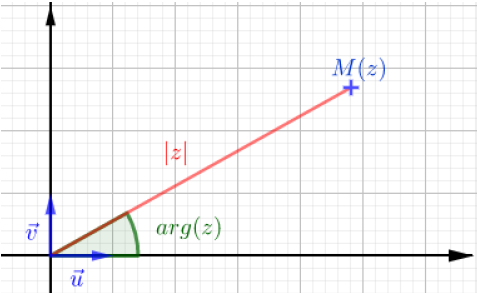
\includegraphics[width = 1 \linewidth]{cplx_arg}
\end{minipage}


\exe Soit $z=3+3i$. On a $|z|=3 \sqrt{2}$ et $ \modu{\arg(z)}{\dfrac{\pi}{4}}{2\pi}$. On peut noter $\arg(z) = \dfrac{\pi}{4} [2\pi]$.

$|i|=1; \arg(i)=\dfrac{\pi}{2} [2 \pi]$.

\props { Soit $z$ un nombre complexe non nul. \vspace*{-0.3cm}
\begin{multicols}{2}
\begin{enumerate}[$(i)$]
\item $z$ est un nombre réel $\iff \arg(z)=0 [\pi]$
\item $z$ est un nombre imaginaire pur $\iff \arg(z)= \dfrac{\pi}{2} [\pi]$
\item $\arg({\overline{z}})=-\arg(z) [2 \pi]$
\item $\arg({-z})=\arg(z)+ \pi [2 \pi]$
\end{enumerate}
\end{multicols}\vspace*{-0.3cm}
}




\begin{minipage}{0.6 \linewidth}
\section{Forme trigonométrique d'un nombre complexe}

%\subsection{Définition}

\prop{Soit $z=a+ib$ un nombre complexe non nul.

On pose : $\theta = \arg(z)$.

On a alors : $a=|z| \cos(\theta)$ et $b=|z| \sin(\theta)$.
}
\end{minipage}
\begin{minipage}{0.35 \linewidth}
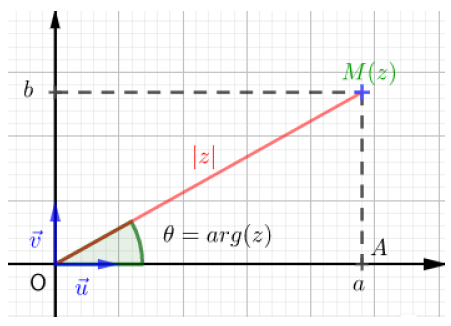
\includegraphics[width = 1 \linewidth]{cplx_geo}
\end{minipage}


\dem Dans le triangle $OAM$ rectangle en $A$ on utilise la trigonométrie de collège.

On a $\cos(\theta)=\dfrac{a}{|z|}$ et $\sin(\theta)=\dfrac{b}{|z|}$.

\defi{On appelle forme trigonométrique d'un nombre complexe non nul l'écriture :

$z=|z|(\cos(\theta)+i \sin(\theta))$ avec $\theta = \arg(z)$.}


\prop{Deux nombres complexes non nuls sont égaux si, et seulement si, ils ont même module et même
argument (modulo $2\pi$).}

\dem 

$\bullet$ Si $z=z'$ implication triviale.

$\bullet$ Réciproque : Si $\left\lbrace \begin{array}{l} |z|=|z'| \\ \arg(z)=\theta=\arg(z')=\theta'[2\pi]  \end{array} \right.$
Alors $z=|z|(\cos(\theta)+i \sin(\theta))=|z'|(\cos(\theta')+i \sin(\theta'))=z'$.



\exe Écrire le nombre complexe $z= \dfrac{\sqrt{2}}{2}+i \dfrac{\sqrt{6}}{2}$ sous sa forme trigonométrique.

\textit{Méthodologie :}

$\bullet$ On commence par calculer le module de $z$

$\bullet$ On calcule $\dfrac{z}{|z|}$ pour identifier la partie réelle de et sa partie imaginaire.

$\bullet$ $|z|= \dots = \sqrt{2}$.

$\bullet$ $\dfrac{z}{|z|}= \dots = \dfrac{1}{2} + i \dfrac{\sqrt{3}}{2}$.

On cherche donc un argument tel que $\cos(\theta)=\dfrac{1}{2}$ et $\sin(\theta)=\dfrac{\sqrt{3}}{2}$.

Parmi les valeurs remarquable on a $\cos(\dfrac{\pi}{3})=\dfrac{1}{2}$ et $\sin(\dfrac{\pi}{3})=\dfrac{\sqrt{3}}{2}$.

D'où $\dfrac{z}{|z|} = \cos(\dfrac{\pi}{3}) + i \sin(\dfrac{\pi}{3})$ puis $z=\sqrt{2} \left(\cos(\dfrac{\pi}{3}) + i \sin(\dfrac{\pi}{3}))\right)$






%\medskip
%
%\subsection{Propriétés}
%
%\props{Soient $z$ et $z'$ deux nombres complexes non nuls et entier naturel non nul.
%
%\renewcommand{\arraystretch}{2} 
%
%\begin{center}
%\begin{tabularx}{0.8 \linewidth}{|M|M|M|}
%\hline 
% & Modules & Arguments \\ 
%\hline 
%Produit & $|zz'|=|z||z'|$ & $\arg(zz')=\arg(z)+arg(z')$ \\ 
%\hline 
%Puissance & $|z^n|=|z|^n$ & $\arg(z^n)=n \arg(z)$ \\ 
%\hline 
%Inverse & $\left| \dfrac{1}{z} \right|=\dfrac{1}{|z|}$ & $\arg\left(\dfrac{1}{z}\right)=-\arg(z)$ \\ 
%\hline 
%Quotient & $\left| \dfrac{z}{z'} \right|=\dfrac{|z|}{|z'|}$ & $\arg\left(\dfrac{z}{z'}\right)=\arg(z)-\arg(z')$ \\ 
%\hline 
%\end{tabularx} 
%\end{center}
%
%}
%

%
%
%\section{Ensemble $\U$ des nombres complexes de module 1}
%
%\subsection{Cercle trigonométrique}
%
%
%\subsection{Stabilité de $\U$}
%
%
%



\end{document}	







